%%%%%%%%%%%%%%%%%%%%%%%%%%%%%%%%%%%%%%%%%%%%%%%%%%%%%%%%%%%%%%%%%%%%%%%%%%%%%%%%
%2345678901234567890123456789012345678901234567890123456789012345678901234567890
%        1         2         3         4         5         6         7         8

\documentclass[letterpaper, 10 pt, conference]{ieeeconf}  % Comment this line out if you need a4paper

%\documentclass[a4paper, 10pt, conference]{ieeeconf}      % Use this line for a4 paper

\IEEEoverridecommandlockouts                              % This command is only needed if 
                                                          % you want to use the \thanks command

\overrideIEEEmargins                                      % Needed to meet printer requirements.

% See the \addtolength command later in the file to balance the column lengths
% on the last page of the document

% The following packages can be found on http:\\www.ctan.org
%\usepackage{graphics} % for pdf, bitmapped graphics files
%\usepackage{epsfig} % for postscript graphics files
%\usepackage{mathptmx} % assumes new font selection scheme installed
%\usepackage{times} % assumes new font selection scheme installed
%\usepackage{amsmath} % assumes amsmath package installed
%\usepackage{amssymb}  % assumes amsmath package installed



\usepackage{amsmath,amssymb}
\usepackage{tikz,hyperref,graphicx,units,subfig}
\usepackage{sidecap,wrapfig}
\usepackage[ruled,vlined]{algorithm2e}
\DeclareMathOperator*{\argmin}{arg\,min}
\DeclareMathOperator*{\argmax}{arg\,max}
\newcommand{\abs}[1]{\lvert#1\rvert} 
\newcommand{\norm}[1]{\lVert#1\rVert}
%\newcommand{\suchthat}{\mid}
\newcommand{\suchthat}{\ \big|\ }
\newcommand{\bd}{\mathbf{d}}
\newcommand{\bn}{\mathbf{n}}
\newcommand{\bp}{\mathbf{p}}
\newcommand{\bw}{\mathbf{w}}
\newcommand{\by}{\mathbf{y}}
\newcommand{\bx}{\mathbf{x}}
\newcommand{\bz}{\mathbf{z}}
\newcommand{\bbf}{\mathbf{f}}
\newcommand{\bzero}{\mathbf{0}}
\newcommand{\bG}{\mathbf{G}}
\newcommand{\bA}{\mathbf{A}}
\newcommand{\bW}{\mathbf{W}}
\newcommand{\bX}{\mathbf{X}}
\newcommand{\mX}{\mathcal{X}}
\newcommand{\mD}{\mathcal{D}}
\newcommand{\mN}{\mathcal{N}}
\newcommand{\mW}{\mathcal{W}}
\newcommand{\mF}{\mathcal{F}}
\newcommand{\bZ}{\mathbf{Z}}

\newcommand{\bfc}{W}
\newcommand{\Qinf}{Q_{\infty}}
\newcommand{\st}[1]{_\text{#1}}
\newcommand{\rres}{r\st{res}}
\newcommand{\pos}[1]{(#1)^+}
\newcommand{\depth}{\operatorname{depth}}
\newcommand{\dist}{\operatorname{dist}}
\newcommand{\convhull}{\operatorname{ConvexHull}}
\newcommand{\minksum}{\operatorname{MinkowskiSum}}



\title{\LARGE \bf
Grasp Metric for Shape Uncertainity with Gaussian Proccess Implicit Surface Representation (Not Finished Work) }


\author{Michael Laskey*, Zoe McCarthy*, Sachin Patil, Pieter Abbeel, and Ken Goldberg}% <-this % stops a space

\newtheorem{theorem}{Theorem}

\begin{document}



\maketitle
\thispagestyle{empty}
\pagestyle{empty}


%%%%%%%%%%%%%%%%%%%%%%%%%%%%%%%%%%%%%%%%%%%%%%%%%%%%%%%%%%%%%%%%%%%%%%%%%%%%%%%%



%%%%%%%%%%%%%%%%%%%%%%%%%%%%%%%%%%%%%%%%%%%%%%%%%%%%%%%%%%%%%%%%%%%%%%%%%%%%%%%%
\section{Introduction}

\vspace{10pt}
 A number of metrics have been proposed to evaluate form and force closure with scalar quality measures for grasping \cite{bicchi2000}.  Many modern 3d sensors give noisy point clouds as output, so shape uncertainty is a common problem \cite{singhbigbird}. As shown in Fig. \ref{fig:noisy data}, the noise in our measurements of object shape can greatly change the surface normals and contact points, which are the parameters that most grasp metrics rely on.  However, only recently have people started looking into a metric's robustness to uncertainty. Prior work by Zheng et al \cite{zheng2005}, looked at how to efficiently include uncertainty in friction coefficient and movement of gripper arm. However, they assumed a known surface of the object.
 
We use Gaussian Processes \cite{rasmussen2006} to convert the point cloud measurements into an implicit surface with uncertainty in the shape.
We assume friction is at the contact points. 
The wrench-space Ferrari-Canny force closure quality measure \cite{ferrari1992} calculates the maximum disturbance that can be resisted given bounds on the contact forces.
%\section{Goals and Current Progress}
We are working to extend this metric to incorporate shape uncertainty.
For our grasping model, we make a simplifying assumption that each gripper approaches the object along a fixed line of action and thus the contact points lie on this line.
We would like to analyze the induced distributions over grasp parameters and the Ferrari-Canny metric.
Specifically, we would like to answer the following question:
What is the probability of achieving force closure under the given grasp approach directions and implicit surface distribution?
So far, we have explicit formulas for the distributions of the contact points along the line of action and surface normal vectors and the expected center of mass of the object to be grasped.
We are thoroughly investigating utilizing recent results on a Lipschitz constant for the Ferrari-Canny metric \cite{pokorny2013classical} in order to prove probabalistic bounds on the change in grasp quality under shape uncertainty.
We are also investigating efficient ways to calculate the distributions on the grasp parameters and ways to update them quickly with new observations.


\begin{figure}[ht!]
\centering
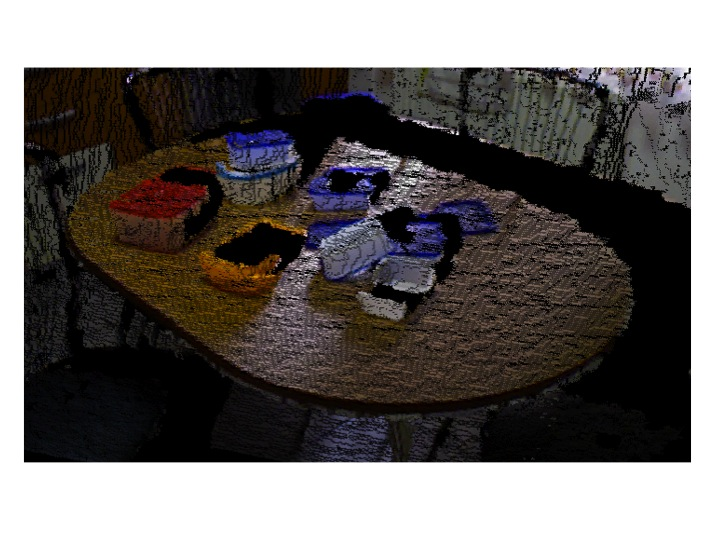
\includegraphics[scale = 0.3]{figures/Slide2.jpg}
\caption{An example of the noise from a Kinect-like sensor}
\vspace*{-10pt}
\label{fig:noisy data}
\end{figure}


\section{Gaussian Process Primer}
%\textbf{TODO:FIX THIS SECTION AND MAKE NOTATION CONSISTENT}
 Gaussian processes (GPs) are widely used in machine learning as a nonparametric regression method for estimating continuous functions from sparse and noisy data \cite{rasmussen2006}.
In a GP, a training set consists of input vectors $\mX = \{\bx_1, \ldots, \bx_n\}, ~\bx_i \in \mathbb{R}^d$, and corresponding observations $\by = \{y_1, \ldots, y_n\}$.
The observations are assumed to be noisy measurements from the unknown target function $f$:
\begin{equation}
y_i = f(\bx_i) + \epsilon,
\end{equation}
where $\epsilon \sim \mN(0,\sigma^2)$ is Gaussian noise in the observations.
A zero-mean Gaussian process is completely specified by a covariance function $k(\cdot,\cdot)$, also referred to as a kernel.
Given the training data $\mD = \{\mX, \by\}$ and covariance function $k(\cdot,\cdot)$, the posterior density $p(f_*|\bx_*,\mD)$ at a test point $\bx_{*}$ is shown to be \cite{rasmussen2006}:
\begin{equation}
  p(f_*|\bx_*,\mD) 
  \sim 
  \mN\big(k(\mX,\bx_*)^{\intercal}(K + \sigma^2I)^{-1}\by,
\end{equation}
\[
  k(\bx_*,\bx_*)-k(\mX,\bx_*)^{\intercal}(K+\sigma^2I)^{-1}k(\mX,\bx_*)\big), \label{eq:GPposterior}
\]
where $K \in \mathbb{R}^{n \times n}$ is a matrix with entries $K_{ij} = k(\bx_i,\bx_j)$ and $k(\mX,\bx_*) = [k(\bx_1,\bx_*),\ldots,k(\bx_n,\bx_*)]^{\intercal}$. 

The choice of kernel is application-specific, since the function $k(\bx_i,\bx_j)$ is used as a measure of correlation between states $\bx_i$ and $\bx_j$.
A common choice is the squared exponential kernel:
\begin{equation}
k(\bx_i,\bx_j) 
=
\nu^2\exp(-\frac{1}{2}(\bx_i - \bx_j)^{\intercal}\Lambda^{-1}(\bx_i - \bx_j))
\end{equation}
where $\Lambda= \text{diag}(\lambda_1^2,\ldots,\lambda_d^2)$ are the characteristic length scales of each dimension of $\bx$ and $\nu^2$ describes the variability of $f$.
The vector of hyper-parameters $\boldsymbol{\theta} = \{\sigma,\nu,\lambda_1,\ldots,\lambda_d\}$ is chosen or optimized during the training process by minimizing the log likelihood $p(\by|\mX,\boldsymbol{\theta})$ \cite{rasmussen2006}.

%\section{Related Work}

\section{Problem Definition}

The objective of our algorithm is to provide an expected quality of grasp, $Q_l^-(\bar{g})$ \cite{ferrari1992}, and the probability $\zeta$ of not obtaining force closure. 

Given a grasp $g$ on an object, we can define it by the following tuple $g = \lbrace \textbf{c}_1,...,\textbf{c}_m,\textbf{n}_1,...,\textbf{n}_m,\textbf{z},\tau\rbrace$. We have a set $I$ of $m$  point contacts and surface normal on the object where $i \in I$s is located at $c_i$ with surface normal $n_i$. The object has a center of mass $z$ and friction coefficient $\tau$.

Since we have uncertainty in the shape we only have a distribution on the grasp parameters, hence $p(g) = \lbrace p(\textbf{c}_1),...,p(\textbf{c}_m),p(\textbf{n}_1),...,p(\textbf{n}_m),\bar{\textbf{z}},\tau \rbrace$. We note that $\tau$ is considered known and $\bar{z}$ is only the expected center of mass. In section \ref{sec:distgrasp}, we demonstrate how to efficiently compute this distribution. 

With distribution on $p(g)$ we then use recent results on a Lipschitz constant for Ferrari-Canny Metric \cite{pokorny2013classical} to provide $\zeta$ or the probability the grasp will lose force closure and the expected quality of the grasp $Q_l^-(\bar{g})$, where $\bar{g} = \lbrace \bar{\textbf{c}}_1,...,\bar{\textbf{c}}_m,\bar{\textbf{n}}_1,...,\bar{\textbf{n}}_m,\bar{\textbf{z}},\tau \rbrace$. Details of this computation can be found in section \ref{sec:bound}.

\section{Distribution of Grasp Parameters}
\label{sec:distgrasp}

 For the following derivations we introduce the following,
 $\theta(x) = \lbrace \mu(x),\Sigma(x) \rbrace$, where $\theta(x)$ is a tuple consisting of the mean and covariance functions given by the trained GPIS model \cite{rasmussen2006} . 
 
 To calculate $p(g)$, we assume a gripper contacts approaches along a line of action, or a 1-dimensional curve in the work space, defined by $\gamma(t)$. See Fig \ref{fig:line_of_action}, for a detailed illustration. Each gripper contact is defined by a line of action, so we assume the following tuple is provided $\Gamma = \lbrace \gamma_1(t),...,\gamma_m(t) \rbrace$, these approach trajectories are then used to compute a distribution on grasp parameters. 
 


We assume a bounded rectangular workspace $\mathcal{R}$.
The line segment has endpoints $a,b$ that are defined as the start of the gripper and the intersection of the line with the end of the workspace respectively, as shown in Fig. 
 \ref{fig:line_of_action}.

 We also define the  level set function as $f(x): \mathbb{R}^d \rightarrow \mathbb{R}$ and an implicit surface as $\mathcal{S} = \{ x \ | \ f(x) = 0 \}$.


\begin{figure}[ht!]
\centering
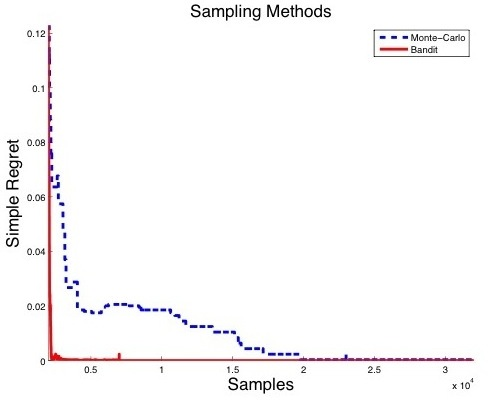
\includegraphics[scale = 0.3]{figures/Slide1.jpg}
\caption{Parametrized Line of Action along an object}
\vspace*{-10pt}
\label{fig:line_of_action}
\end{figure}
\textbf{TODO:MORE DESCRIPTIVE GRAPHIC}
\subsection{Distribution on Contact Points} The probability distribution along the line $\gamma(t)$ is given by the following:

\begin{equation}
p\big(f(\gamma(t))|\theta(\gamma(t)): \forall t \in [a,b] \big) 
=
\mN(\mu_{a:b},\Sigma_{a:b})
\end{equation}

This gives the distributions along the entire line of action in the workspace, however we want to compute the joint distribution   $p\big(\textbf{c}_i= \gamma(t)\big) = p\big(f(\gamma(t))=0, f(\gamma(\tau))> 0: \forall \tau \in [0,t)\big)$. Hence we want to know at a point what the distribution  is that it is at the surface and the probability that all points before are before the surface, this avoids the problem of the distribution producing multiple modes for each intersection with the surface. We now derive a  this distribution 

\begin{align*}
p\big(\textbf{c}_i = \gamma(t)\big) &\propto p\big(f(\gamma(t)) = 0\big)\\
               &*P\big(f(\gamma(\tau)) > 0 | f(\gamma(t)) = 0: \forall \tau \in [0,t)\big)
\end{align*}

Using the first product in the equation can be computed easily using the marginalization of a multivariate Gaussian distribution and the second one can be rewritten by conditioning the distribution \cite{petersen2008matrix}. 

\begin{align*}
p_c\big(f(\gamma(\tau)): \forall \tau \in [0,t)\big) = p\big(f(\gamma(\tau))  | f(\gamma(t)) = 0\big)  
\end{align*}


It is now clear that the following can be said

\begin{align*}
p\big(\textbf{c}_i = \gamma(t)\big) &= \frac{1}{\eta} p(f\gamma(t) = 0) \\
				   &*P_c\big(f(\gamma(\tau)) > 0): \forall \tau \in [0,t)\big)			 
\end{align*} 

The second product term can be efficiently evaluated by looking up the cumulative distribution of a multivariate Gaussian, which is common in most software packages \cite{matlab}.

\subsection{Distribution on Surface Normals} 
The distribution of surface normals $p(\textbf{n}_i = \textbf{k})$ can be calculate as follows.
First we assume that some function exists $h(x) = \lbrace \mu_{\nabla}(x), \Sigma_{\nabla}(x) \rbrace$, hence given a point $\bf{x}$ it returns the parameters for a Gaussian distribution around the gradient.
this function can be computed via learning the gradient \cite{solak2003derivative} or analytical differentiation of $f(x)$.
We note that both methods yield a Gaussian distribution.
We now demonstrate how to marginalize out the contact distribution and compute $p(\textbf{n}_i = \textbf{k})$\\

From our distribution on contact points and Bayes rule we can compute the following: 

\begin{equation}
p(\textbf{c}_i = \gamma(t), \textbf{n}_i = \textbf{k}) = p\big(\textbf{n}_i = \textbf{k} | h(\gamma(t))\big)*p\big(\textbf{c}_i = \gamma(t)\big)
\end{equation}

Now we can marginalize out the distribution on contacts:

\begin{equation}
p(\textbf{n}_i = \textbf{k}) = \int_a^b  p \big(\textbf{n}_i = \textbf{k} | \textbf{c}_i = \gamma(t) \big)*p(\textbf{c}_i = \gamma(t)) dt
\end{equation}

\begin{equation}
p\big(\textbf{n}_i = \textbf{k}\big) = \int_a^b  p \big(\textbf{n}_i = \textbf{k} | h(\gamma(t))\big)*p\big(\textbf{c}_i = \gamma(t)\big) dt
\end{equation}

We approximate this by uniformly sampling the integral along the function $\gamma(t)$ and achieve the following: 

\begin{equation}
p\big( \textbf{n}_i = \textbf{k} \big) = \sum_T  p \big( \textbf{n}_i = k | h(\gamma(t)) \big) *p\big(c_i = \gamma(t)\big) dt
\end{equation}


Thus, $p(\textbf{n}_i = \textbf{k})$ is approximated by a Gaussian Mixture Model.

\subsection{Expected Center of Mass} 

We define the quantity $\mathcal{D}(x) = \int_{-\infty}^{0} p(f(x) =  s \ | \ \theta(x)) ds$ and note that it is equal to the probability that x is interior to the surface under the current observations.
We assume that the object has uniform mass density and then $\mathcal{D}(x)$ is the expected mass density at x.
Then we can find the expected center of mass as:

\begin{equation}
  \bar{z} 
  =
  \frac
    {\int_{\mathcal{R}}x \mathcal{D}(x) dx}
    {\int_{\mathcal{R}}  \mathcal{D}(x) dx}
\end{equation}

which can be approximated by sampling $\mathcal{R}$ uniformly in a voxel grid and approximating the spatial integral by a sum.


\section{Probabilistic Bound on Grasp Metric}
\label{sec:bound}
Following recent work on proving a Lipschitz bound on the Ferrari-Canny Metric \cite{pokorny2013classical}, we prove that an extension is possible to give a probabilistic bound on the change in grasp quality.
We rewrite the results here:

\subsection{Prior Work}

\textbf{TODO:WORK IN PRIOR WORK BETTER}
We follow the notation of \cite{pokorny2013classical} except that their $\mu$ is our $\tau$ since we use $\mu$ to refer to means.  
We re-state some of their central theorems for our use here.
For more detail, refer there.
$Q(g)$ is the exact $L^1$ grasp quality.
It is denoted by the following 

\begin{align}
  Q(g) &= \mbox{max}(0,q(g)) = -d(0,\mbox{Conv}(\{0\} \cup S(g))\\
-d(0,S) &= min_{||z|| = 1} h_{S(z)}\\
h_{S(z)} &= \mbox{sup}_{s\in S}\langle s,z\rangle\\
\end{align}

We denote the Ferrari-Canny version, which approximates the friction cone by a linearized set of wrenches\cite{ferrari1992}, as $Q^-_l(g)$.
The next theorem shows that the linearized wrench set used in Ferrari-Canny calculates a lower bound on $Q(g)$.\\

\begin{theorem}
  \cite{pokorny2013classical}
For any grasp g, we have $0 \leq Q_l^-(g) \leq Q(g)$.
Furthermore, $||Q(g) - Q^-_l(g)|| \rightarrow 0$ as $l \rightarrow \infty$ when $Q_l^-(g)$ is computed using a uniform approximation of the friction cones with $l$ edges. \\
\end{theorem}

The next theorems are used to show that $Q$ is Lipschitz continuous.

\begin{theorem}
\label{lemma35}
  \cite{pokorny2013classical}
For $w \in \mathbb{R}^3$, we have, for $n \in \mathbb{S}^2$ and for friction coefficient $\mu > 0$, 

\begin{align}
\mbox{sup}_{x \in C(n)} \langle x,w \rangle = \langle n,w \rangle + \tau||n \times w||
\end{align}

Hence, for $u = (a,b) \in \mathbb{R}^3 \times \mathbb{R}^3 = \mathbb{R}^6$, we have 

\[
h_{W_i(g)}(a,b) =
 \langle n_i,a+b\times(c_i-z)\rangle +
\]
\begin{align}
 +\tau ||n_i \times (a+b\times(c_i-z))||
\end{align}

\end{theorem}

\begin{theorem}
  \cite{pokorny2013classical}
We have \\

\begin{align}
q(g) 
=
\min_{u\in \mathbb{R}^6, ||u|| =1} h_{S(g)}(u) 
=
\end{align}
\[
\min_{u\in \mathbb{R}^6, ||u|| =1} \max_{i=1,...,m} h_{W_i(g)}(u),
\]

where $h_{S(g)}$ is convex on $\mathbb{R}^6$.
$q$ is invariant under fixed translation of the grasp center and contact positions.
Furthermore, let $\mathbb{B}(r) = \lbrace x \in \mathbb{R}^3 : ||x|| \leq r \rbrace$.
Then $q$ is Lipschitz continuous on grasps with $m$ contact points lying in the set $X = \lbrace (c_1, \dots, c_m,n_1, \dots,n_m,z) : (c_i-z) \in \mathbb{B}(r), n_i \in \mathbb{S}^2 \rbrace$ with a Lipschitz constant given by $L= (1+\mu)(1+r)$ and where we use distance measure 

\[
  d(g,g') = \sum_i ||(c_i-z)-(c_i'-z')|| + \sum_i ||n_i - n_i'||.
\]

We hence have 

\[
|q(g) - q(g')| \leq Ld(g,g'),\  \forall g,g' \in X.
\]

Since $Q(g) = \max(0,q(g))$, $Q$ is also Lipschitz continuous with the same constant $L$ on $X$. 
\end{theorem}

Setting $l_{i,a,b} = h_{W_i(g)}(a,b)$, we have for $||(a,b)|| \leq 1$ that is $|l_{i,a,b}(g) - l_{i,a,b}(g')|$ is bounded by $|\langle n_i,a+b\times (c_i-z)\rangle - \langle n_i',a+b\times(c_i'-z')\rangle|+\mu|||n_i \times (a+b \times (c_i -z))|| - ||n_i \times (a + b \times (c_i' - z')) |||$, using Theorem \ref{lemma35}.
By using the following facts $||a|| \leq 1$, $||b|| \leq 1$, $||v \times w || \leq ||w||||v||$, $|\langle v,w\rangle | \leq ||v||||w||$, we obtain:  

\begin{align*}
|l_{i,a,b}(g) - l_{i,a,b}(g')| &\leq ||n_i - n_i'||(1+||c_i - z||) \\
					&+ ||(c_i - z)-(c_i'-z')|| \\
					&+ \tau(||n_i - n_i'||(1+||c_i - z||)\\
					&+||(c_i - z)-(c_i'-z')||)
\end{align*}

\subsection{Our Extension}
We now define the concept of a probabilistic bound by functions $\sigma_i(\zeta) = \lbrace\Delta \textbf{r}_{i,\zeta}, \Delta \textbf{n}_{i,\zeta}\rbrace$. Given a probability $\zeta$, $\sigma_i$ returns the tuple denoting the maximum change in grasp parameter from the mean in the distribution for that probability. $\Delta \textbf{n}_i$ is the change in surface normal and $\Delta \textbf{r}_i$ is the change in moment arm defined as $\textbf{r}_i = \textbf{c}_i - \bar{\textbf{z}}$.
Formally, this is defined as:

\[
  \sigma_i(\zeta)
  =
  \min_{\mathbb{R}_+} \textbf{d}
\]

\[
  s.t. \ \ \left[ \int_{\mathbb{B}([\bar{t},\bar{\textbf{n}}], d)} p(\textbf{n}_i = \textbf{k},\textbf{c}_i=\gamma(t)) d[t,\textbf{k}] \right] \geq \zeta
\]



We now write the above bound as follows for a given $\sigma_i(\zeta)$: 

 \begin{align*}
|l_{i,a,b}(g) - l_{i,a,b}(g')| & \leq ||\Delta \textbf{n}_{i,\zeta}||(1+||\bar{\textbf{r}}_i||) + ||\Delta{\textbf{r}_{i,\zeta}}(\zeta)|| \\
                                      &+ \tau(||\Delta \textbf{n}_{i,\zeta}||(1+||\bar{\textbf{r}}_i||)+||\Delta \textbf{r}_{i,\zeta}||)
\end{align*}

For convenience we rewrite the bound on a given set of grasp parameters as : 

 \begin{align*}
b_i(\zeta) &= ||\Delta \textbf{n}_{i,\zeta}||(1+||\bar{\textbf{r}}_i||) + ||\Delta{\textbf{r}_{i,\zeta}}(\zeta)|| \\
                                      &+ \tau(||\Delta \textbf{n}_{i,\zeta}||(1+||\bar{\textbf{r}}_i||)+||\Delta \textbf{r}_{i,\zeta}||)
\end{align*}

To provide an upper bound overall contact parameters we introduce the following: 

\begin{align}
b(\zeta)  = \max_{i} b_i(\zeta)
\end{align}

To prove if  this bound is preserved on

 \begin{align}
 q(g) = \min_{(a,b) \in \mathbb{R}^6, ||u||=1} \max_{i=1,..,m} l_{i,a,b}(g)
 \end{align}
 
we turn to the general case.
$\lambda(x) = \mbox{inf}_{\alpha \in A} f_\alpha(x)$ and $\lambda(x) = \mbox{sup}_{\alpha \in A} f_\alpha(x)$ are bounded with $b(\zeta)$ if $f_\alpha(x)$ for all $\alpha$ is bounded with $b(\zeta)$ and $\lambda(x)$ is bounded.
Since our bound is invariant to the variables $(a,b)$ and we take the maximum set of parameters $i$.
We can ensure that is true.

Lastly if one wants to find the probability they would lose force closure, they can simply solve the following 

\[
  \zeta
  =
  \argmin_{\zeta} b(\zeta)
\]

\[
  s.t. \ \  b(\zeta) \geq q(\bar(g))
\]

This would be pretty computationally expensive, so still a work in progress. \textbf{TODO:MAKE THIS EFFICIENT}

\bibliographystyle{ieeetr}
\bibliography{references}

\end{document}
